\chapter{Lösungsansatz}
\label{ch:loesungsansatz}

\section{Selbstlernende KI mithilfe von Trainingsdaten}
\label{sec:selbstlernende-ki-trainingsdaten}

Zunächst war eine Überlegung, ob eine \ac{KI} mithilfe generierter Daten trainiert werden kann.
Je nach vorliegender Spielsituation würde die \ac{KI}, \bspw unter Einsatz von neuronalen Netzen, eigene Entscheidungen treffen können.
Dieser Ansatz bringt jedoch das Problem mit sich, gute Trainingsdatensätze besitzen zu müssen.
Bei einer maximalen Anzahl von sechs Spielern im Spiel \texttt{spe\_ed} und fünf unterschiedlichen Aktionen gibt
es sehr viele Möglichkeiten, wie ein Spiel verlaufen kann.
Dabei entsteht das Problem, beurteilen zu müssen, welche Spielsituationen und welche Spielverläufe als Trainingsdaten
gut geeignet sind, sodass die gesamte Komplexität des Spiels in den Trainingsdaten abgebildet wird.
Ist es nicht möglich, eine ausreichend umfangreiche Menge an Daten generieren zu können, besteht die Gefahr, dass eine
damit trainierte \ac{KI} deutlich schlechtere Entscheidungen trifft als eine Implementierung, die auf simpleren und
programmatisch vorgegebenen Heuristiken basiert.
Aufgrund dessen fiel die Entscheidung, zunächst Lösungsansätze ohne eine selbstlernende \ac{KI} zu implementieren.
Diese Strategie hatte für uns den Vorteil, mithilfe einfacherer Lösungsansätze die Komplexität und auftretenden Probleme
im Spielverlauf besser kennenlernen zu können.

\section{Lösungsansätze ohne selbstlernende KIs}
\label{sec:loesungsansatz-ohne-selbstlernende-kis}

Bei dem Ansatz, Strategien fest in Code zu implementieren, hatten wir mehrere unterschiedliche Ideen,
die nachfolgend beschrieben werden.
Ziel war es hierbei, Teilprobleme zu erkennen und zu lösen, mit der Intuition diese unterschiedlichen \ac{KI}s
kombinieren zu können.
Die nachfolgend beschriebenen \ac{KI}s und die Abhängigkeiten dieser können in \Anhang{fig:klassendiagramm-AIs}
nachvollzogen werden.
Die Mehrfachvererbungen, wie sie im UML-Klassendiagramm dargestellt werden, wurden in der Implementierung durch die
Verwendung von Python als Programmiersprache genau so umgesetzt.

\subsection{RandomAI}
\label{subsec:random-ai}

Die \Code{RandomAI} ist unsere erste lauffähige KI gewesen und unser Maß für die einfachste \ac{KI}.
Diese stellt zwar keinen wirklichen Lösungsansatz dar, diente jedoch als Einstieg und um erste Probleme zu erkennen.
Durch die \Code{RandomAI} ist uns das grundlegende Problem aufgefallen, dass sich die \ac{KI} selber tötet.
Folglich wird die Minimal- und Maximalgeschwindigkeit überschritten, das Spielfeld verlassen oder in vorhandene Spuren
gefahren, mit denen eine Kollision vermeidbar gewesen wäre.

\subsection{NotKillingItselfAI}
\label{subsec:notkillingitself-ai}

Aufgrund des beschriebenen Problemes der \Code{RandomAI} haben wir uns dafür entschieden, die \Code{NotKillingItselfAI}
zu implementieren.
Die \ac{KI} soll aus allen Aktionen eine zufällige Aktion auswählt, die sie nicht direkt verlieren lässt.
Dazu wird für jede mögliche Aktion die Spur berechnet, die entstehen würde und auf Kollisionen überprüft.
Aktionen die eine Kollision hervorrufen werden nicht ausgeführt.
Hierbei bleiben mögliche Aktionen der Gegenspieler zunächst unberücksichtigt. \\

Durch die Implementierung der \Code{NotKillingItselfAI} fiel auf, dass die \ac{KI} sich zwar nicht mehr im unmittelbar
folgenden Zug tötete, jedoch häufig in Sackgassen läuft.
Dieses Problem wird in der \Abbildung{fig:Sackgassen_Problem} verdeutlicht.

\begin{figure}[htb]
    \centering
    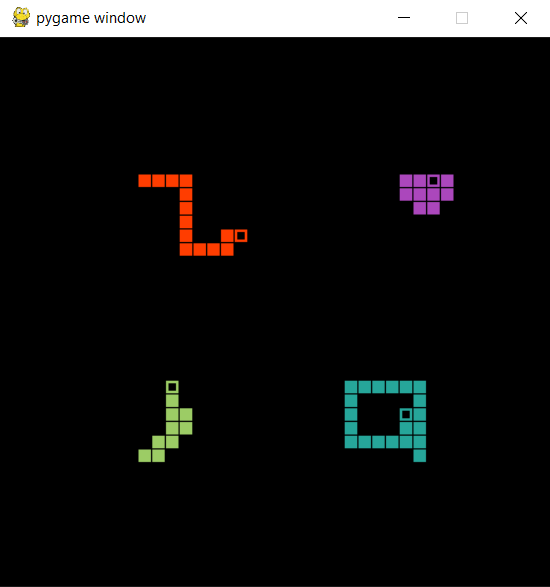
\includegraphics[width=0.6\textwidth]{Bilder/Sackgassen_Problem.png}
    \caption{\Code{NotKillingItselfAI} unten rechts in einer Sackgasse}
    \label{fig:Sackgassen_Problem}
\end{figure}

\subsection{PathfindingAI}
\label{subsec:pathfinding-ai}

Folglich der \Code{NotKillingItselfAI} haben wir einen Lösungsansatz gesucht, welcher das Betreten von Sackgassen
verhindert.
Genutzt wurde die Basis der \Code{NotKillingItselfAI}, sodass nur zwischen überlebenden Aktionen gewählt wird.
Um die Aktionen zu finden, die nicht in eine Sackgasse läuft, haben wir uns für einen Lösungsansatz zum Finden von
Pfaden entschieden.
Dazu wird eine konfigurierbare Anzahl zufälliger Koordinaten generiert, auf denen sich bisher kein Spieler befindet.
Anschließend wird für jede Aktion geprüft, zu wie vielen der Koordinaten, nach der Ausführung der Aktion noch ein
möglicher Pfad existiert.
Die Aktion, die die höchste Anzahl Koordinaten erreichen kann, führt mit höchster Wahrscheinlichkeit
nicht in eine Sackgasse und wird ausgewählt.
In der \Abbildung{fig:sackgasse-pfade} wird dies grafisch verdeutlicht.
Die gelben Quadrate stellen die zu erreichenden Koordinaten dar und somit ist nach der Aktion turn\_left nur noch ein
Pfad erreichbar und nach Ausführung der Aktion turn\_right hingegen drei Pfade.
Folglich wählt die \Code{PathfindingAI} die Aktion turn\_right.

\begin{figure}[htb]
    \centering
    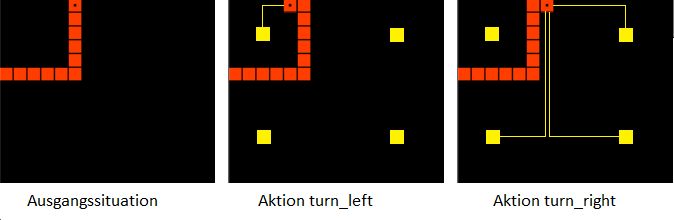
\includegraphics{Bilder/pathfinding_example.png}
    \caption{Auswirkung unterschiedlicher Aktionen auf die erreichbaren Pfade}
    \label{fig:sackgasse-pfade}
\end{figure}

Bei diesem Lösungsansatz arbeiten wir lediglich mit der Wahrscheinlichkeit, dass wir nicht in eine Sackgasse laufen.
Dies liegt dem Problem zugrunde, dass wir die Implementierung eines Algorithmus zum tatsächtichen Erkennen von
Sackgassen oder abgesperrten Gebieten als schwieriger erachteten. \\

Wir haben die Python-Bibliothek \Code{pathfinding} verwendet, die bereits unterschiedliche Algorithmen zum Finden von
Pfaden in einem Graphen bietet.
Die Entscheidung, welcher Algorithmus zum Finden eines Pfades verwendet wird, hat eine große Auswirkung auf die
Performance der \Code{PathfindingAI}.
Der Algorithmus stellt den Flaschenhals dar, da dieser je nach Konfiguration mehrere hundert bis tausend mal pro
Zug ausgeführt werden muss.
Wir haben unterschiedliche Algorithmen, die die Bibliothek zur Verfügung stellt, hinsichtlich ihrer Ausführungsdauer verglichen und uns folglich für die
Verwendung vom Best-First-Algorithmus entschieden.
Bei dem Vergleich wurde in 50 unterschiedlichen Spielsituationen jeweils 200 Pfade für jede mögliche Aktion gesucht, um
den schnellsten Algorithmus zu finden.
Die durchschnittlichen Ausführungzeiten auf unserem Testrechner können der
\Tabelle{tab:ausfuehrungsdauer-pfadalgorithmen} entnommen werden.

\begin{table}[htb]
    \centering
    \begin{tabular}{|l|l|}
        \hline
            \textbf{Algorithmus} & {\textbf{Durchschnittliche Ausführungsdauer in Sekunden}} \\ \hline
            BestFirst 		    & 0.740099930763244 \\ \hline
            BiAStarFinder 		& 0.994705820083618 \\ \hline
            AStarFinder 		& 1.257498860359192 \\ \hline
            BreadthFirstFinder  & 1.376600646972656 \\ \hline
            DijkstraFinder		& 2.440193486213684 \\ \hline
    \end{tabular}
    \caption{Ausführungsdauer unterschiedlicher Algorithmen zum Finden von Pfaden}
    \label{tab:ausfuehrungsdauer-pfadalgorithmen}
\end{table}

\subsubsection*{Best-First-Algorithmus}
\label{subsubsec:best-first-algorithm}

Bei dem Best-First-Algorithmus handelt es sich um eine Bestensuche, bei der ein gegebener Graph mit einem Start- und
einem Endpunkt nach einem Pfad durchsucht wird.
Die Strategie der Bestensuche ist es, den vielversprechendsten Knoten als Nächstes zu wählen und von dort aus dann
wiederum die Suche fortzusetzen.
Der Dokumentation zur von uns genutzten Klasse \Code{BestFirst} der Bibliothek \Code{pathfinding} kann entnommen werden,
dass für den Best-First-Algorithmus der A*-Algorithmus genutzt wird und zusätzlich die Heuristik für die Bewertung der
Nachbarknoten geändert wurde.
Als Heuristik zur Berechnung der Distanz zwischen zwei Punkten wird bei diesem Algorithmus die Manhattan-Distanz
genutzt, die die Summe der absoluten Differenzen der x- und y-Koordinaten darstellt. \Vgl{luderer2017misst}

Bei jedem Nachbarknoten des aktuell betrachteten Knotens wird die Manhatten-Distanz zum Start- sowie Endknoten
berechnet.
Summiert ergeben diese beiden Distanzwerte dann eine heuristische Bewertung des Nachbarknotens.
Die Suche wird dann mit dem Knoten fortgesetzt, für den die beste Bewertung errechnet wurde und die umliegenden Knoten
hinsichtlich der Distanzwerte aktualisiert.
Dies wird solange fortgeführt, bis der beste Pfad gefunden oder alle erreichbaren Knoten des Graphen besucht wurden.
\Vgl{cui2011based}

\subsection{SearchTreeAI}
\label{subsec:searchtree-ai}

Sowohl bei der \Code{NotKillingItselfAI} als auch der \Code{PathfindingAI} gibt es weiterhin ein Problem.
Die \ac{KI} errechnet zwar Aktionen, die sie für die nächste Runde überleben lassen, allerdings werden die möglichen
Aktionen der Gegenspieler nicht beachtet und es ist keine Prognose möglich, wie gut diese Aktion in den kommenden Runden
sein könnte.
Ziel der \Code{SearchTreeAI} ist es, dass nur Aktionen berücksichtigt werden, bei denen bereits alle möglichen
gegnerischen Aktionen und dessen Auswirkungen berücksichtigt werden und der eigene Spieler trotzdem überlebt. \\

Unser Lösungsansatz für dieses Problem ist es, mithilfe eines Suchbaums alle möglichen gegnerischen und eigenen
Aktions-Kombinationen eine bestimmte Anzahl Spielzüge in die Zukunft zu simulieren. 
Dabei wird dann nach einem Teilbaum gesucht, bei dem
vorhergesagt werden kann, dass der eigene Spieler unabhängig der von allen anderen Spielern ausgewählten Aktionen nicht
im nächsten Zug stirbt.
Für diese Simulation konnte viel von der in \Kapitel{sec:offline-implementierung} beschriebenen Implementierung
wiederverwendet werden. \\

Diese Idee wird in \Abbildung{fig:SearchTreeAIVisualisierung} visualisiert, wobei es in diesem Beispiel neben dem
eigenen Spieler noch die beiden weiteren Spieler mit den IDs 1 und 2 gibt.
Die Buchstaben an den Pfaden sollen jeweils die simulierte Aktion kennzeichnen.
Der Baum wird von links nach rechts aufgebaut und besteht pro Zug aus zwei Ebenen.
Zuerst wird ausgehend vom aktuellen Spielstand die eigene Aktion des Spielers berechnet und abgebrochen, wenn hier schon
kein Überleben mehr möglich ist.
Im zweiten Schritt wird für jede mögliche Aktion des eigenen Spielers jede mögliche Kombination der gegnerischen
Aktionen simuliert und wiederum das Überleben geprüft. \\

\begin{figure}[htb]
\centering
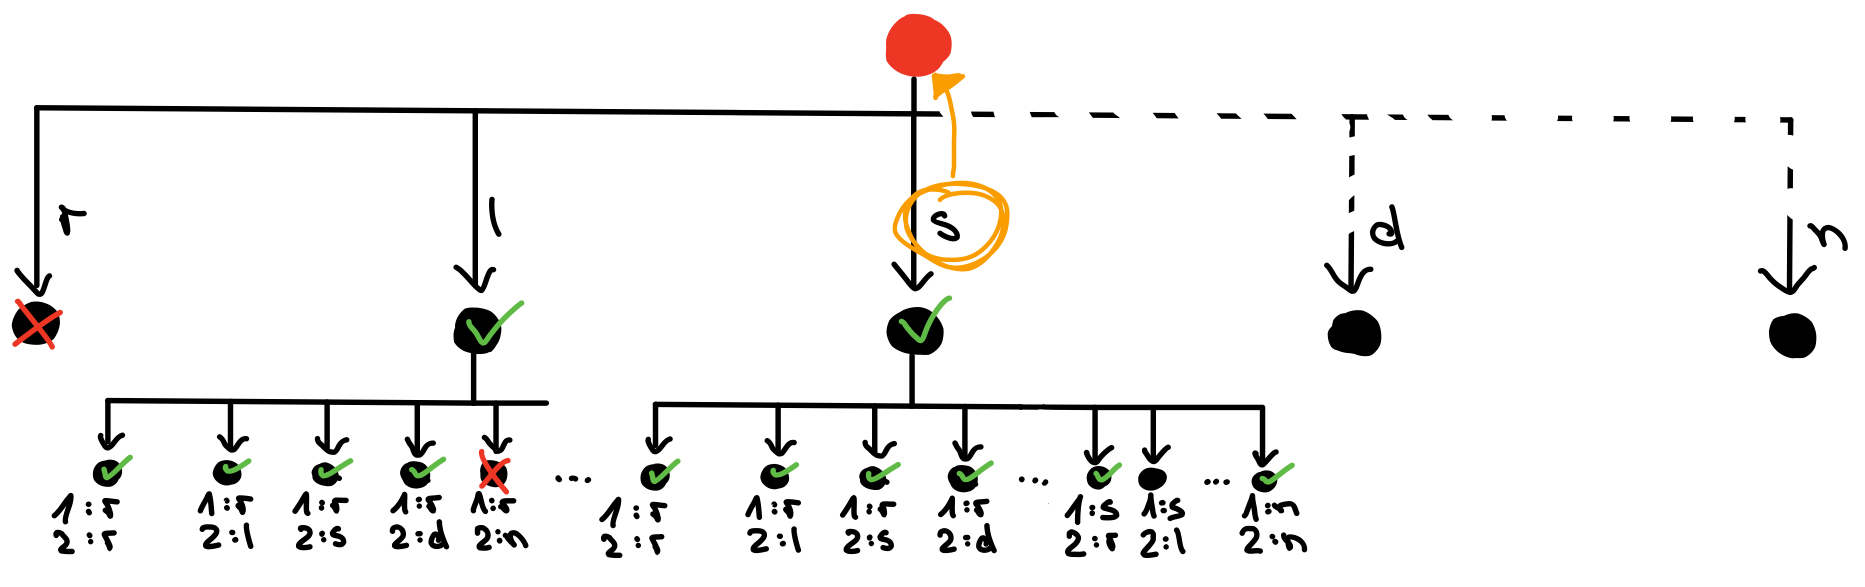
\includegraphics[width=\textwidth]{Bilder/SearchTreeAIVisualisierung.jpg}
\caption{Visualisierung der Idee der \Code{SearchTreeAI}}
\label{fig:SearchTreeAIVisualisierung}
\end{figure}

Gibt es einen Pfad bis zur vorletzten Ebene, nach dem bei der Kombination aller gegnerischen Aktionen immer ein
Überleben auf der untersten Ebene folgt, ist eine Ausgangsaktion gefunden, die in dem aktuellen Zug ausgeführt werden
kann, um in jedem Fall die Anzahl der nächsten berechneten Züge überleben zu können. \\

Ein Problem stellt hierbei allerdings die für jeden Zug extrem stark steigende Anzahl zu berechnender Aktionen dar.
Während bei einem Spiel mit der Maximalzahl von sechs Spielern und fünf möglichen Aktionen die Berechnung von drei Zügen
im schlimmsten Fall $(6 ^ 5) ^ 3 = 470.184.984.576$ Kombinationen umfasst, sind es bei vier Zügen schon
$(6 ^ 5) ^ 4 = 3.656.158.440.062.976$. \\

Da diese Anzahl an Berechnungen in der Zeit bis zum Ablaufen der Deadline nicht durchgeführt werden kann, wurde diese
Anzahl reduziert, indem in die Simulation nicht immer alle Spieler einberechnet werden, sondern nur noch solche,
die sich in einer gewissen Distanz zu dem eigenen Spieler befinden.
Um die Entfernung zwischen dem eigenen und den anderen Spielern unter der Berücksichtigung der bereits belegten Felder
zu errechnen, konnte der bereits beschriebene Algorithmus zum Finden von Pfaden wiederverwendet werden.
Ist dann \bspw nur noch ein weiterer Spieler überhaupt in unmittelbarer Nähe, reduziert sich die Zahl von
$470.184.984.576$ auf lediglich $(2 ^ 5) ^ 3 = 32.768$ Kombinationen.

\subsection{SearchTreePathfindingAI}
\label{subsec:searchtree-pathfinding-ai}

Die \Code{SearchTreePathfindingAI} kombiniert die Stärken der \Code{SearchTreeAI} und der \Code{Pathfinding\-AI}.
Hierbei wird die Entscheidung der \Code{SearchTreeAI} priorisiert.
Dazu werden der \Code{PathfindingAI} zur Berechnung der besten Aktionen nur noch die Aktionen zur Verfügung gestellt, die
durch die \Code{SearchTreeAI} ermittelt wurden.
Dadurch erreichen wir, dass die Aktion mit den meisten Pfaden gewählt wird, die in jedem Fall die nächsten Züge,
entsprechend der gewählten Tiefe des Suchbaums, überleben wird.

Ein Nachteil dieser Variante ist, dass die \Code{SearchTreePathfindingAI} sich durch andere gegnerische Spieler in
seltenen Spielsituationen in Sackgassen zwingen lassen kann.

\subsection{PathfindingSearchTreeAI}
\label{subsec:pathfinding-searchtree-ai}

Die \Code{PathfindingSearchTreeAI} kombiniert ebenso wie die \Code{PathfindingSearchTreeAI} die Stärken der
\Code{SearchTreeAI} und der \Code{PathfindingAI}, priorisiert jedoch die Entscheidungsgrundlage der
\Code{PathfindingAI}.

Die \Code{PathfindingAI} erstellt zunächst eine Liste der Aktionen mit den erreichbaren Pfaden.
Die Liste wird absteigend nach der Aktion sortiert, die die meisten Pfade erreichen kann.
Die \Code{SearchTreeAI} berechnet ebenfalls eine Liste möglicher Aktionen.
Aus diesen beiden Listen muss dann eine Aktion ausgewählt werden, die den beiden Ergebnissen der \ac{KI}s genügt.

Die Priorisierung hinsichtlich der \Code{PathfindingAI} ist so umgesetzt, dass der \Code{PathfindingSearch\-TreeAI} bei
der Initialisierung ein Parameter übergeben wird, der eine Toleranz zwischen 0 und 1 darstellt.
Eine mögliche Aktion der \Code{SearchTreeAI} muss mindestens die maximal mögliche Anzahl an Pfaden multipliziert mit der
Toleranz (\ref{eq:toleranz-pathfinding-searchtree-ai}) erreichen können.

\begin{equation}
\label{eq:toleranz-pathfinding-searchtree-ai}
erreichbare\_Pfade >= maximal\_erreichbare\_Pfade * Toleranz
\end{equation}

Sofern keine Aktion gefunden wird, die in beiden Aktions-Listen vorhanden ist und dieser Formel entspricht, wird die
beste Aktion der \Code{PathfindingAI} gewählt.
Diese Strategie bewirkt, dass sich die \Code{PathfindingSearchTreeAI} nicht in zu kleine Gebiete durch die Gegner
zwingen lässt.
Jedoch besteht das Risiko, eine vermeidbare Kollision zu verursachen.

\subsection{Weitere nicht umgesetzte Lösungsansätze}
\label{subsec:weitere-loesungsansaetze}

Alle bisher beschriebenen Lösungsansätze haben die Eigenschaft, dass sie so lange wie möglich überleben wollen.
Dabei wird jedoch nicht der Ansatz verfolgt, die anderen Mitspieler gezielt dazu zu bringen, kürzer zu überleben als man
selbst.
Nachfolgend werden derartige Lösungsideen beschrieben und erklärt, warum wir uns gegen die Implementierung dieser
entschieden haben. \\

Als ein möglicher Lösungsansatz stand zur Diskussion, die gegnerischen Spieler an den Spielfeldrand zu drängen und ihn somit
zum Verlieren zu zwingen.
Bei diesem Ansatz muss die eigene KI dicht an die gegnerische \ac{KI} fahren, damit diese zu Entscheidungen gezwungen
wird, die nicht optimal sind und ein vorzeitiges Verlieren bedeuten.

Problematisch bei einer zu kleinen Distanz zu den gegnerischen Spielern ist jedoch, dass man den Aktionen der Mitspieler
vertrauen muss.
Es ist notwendig, dass der Gegner kein Risiko eingeht und immer nur Aktionen wählt, die unter Berücksichtigung der
möglichen Aktionen unserer \ac{KI} nicht zum Verlieren führen.
Würde die \ac{KI} nicht dicht an den Gegner heranfahren und einen Sicherheitsabstand einhalten, wäre diese Strategie
unwirksam, denn es bleiben zu viele gute Optionen für den Gegner übrig. \\

Resultierend aus dem Problem, nicht absichtlich zu dicht an Mitspieler heranfahren zu wollen, entstand der Lösungsansatz,
einen Gegner zu umkreisen und somit in ein kleines Gebiet einzusperren.
Dadurch würde man dazu beitragen, dass der Gegner entweder nur noch wenige Züge zur Verfügung hat und den verbleibenden
Platz nutzt, oder einen sechsten Zug mit einer Geschwindigkeit größer zwei nutzen muss, um aus dem begrenzten Feld
wieder heraus zu kommen.
Die Berechnung mit einem sechsten Zug über die umkreisenden Spur zu kommen ist nicht trivial und zudem existiert dazu in
einigen Spielsituationen keine mögliche Option.
Diese Vorteile sprechen zunächst für diesen Lösungsansatz, jedoch bringt er wiederum auch eine erhöhte Gefahr für das
Ausscheiden der eigenen \ac{KI} mit sich.

Um einen gegnerischen Spieler umkreisen zu können, muss eine solche aggressive \ac{KI} in den meisten Fällen schneller sein als
der Gegenspieler.
Dies bedeutet aber auch, dass Geschwindigkeiten erreicht werden müssen, die Löcher in der Spur in jedem sechsten Zug
hinterlassen, wodurch das Umkreisen an Wirkung verlieren würde.
Außerdem hat sich ein hohe Geschwindigkeit bei der Evaluation unserer implementierten Lösungsansätze bereits als
riskant herausgestellt.
Die erhöhte Geschwindigkeit sorgt dafür, dass häufig nur wenige oder keine Aktion zur Auswahl stehen, die im
nächsten Spielzug nicht zum Verlieren führen.

Daher steigt die Wahrscheinlichkeit, dass die eigene \ac{KI} durch ihr agressives Verhalten frühzeitig ausscheidet.
Dieses Risiko gepaart mit dem Problem der Löcher in der Umkreisung hat dafür gesorgt, dass auch dieser Lösungsansatz
nicht implmentiert wurde. \\

Aufgrund der genannten Probleme haben wir uns dagegen entscheiden, eine \ac{KI} zu implementieren, die proaktiv für das
Ausscheiden anderer Spieler sorgt, da sich das Risiko für das eigene Ausscheiden zu stark erhöht.

\section{Vorgehen zur Auswahl der besten Strategie}
\label{sec:vorgehen-strategieauswahl}

\todo{Kapitel ausformulieren}
